%%%%%%%%%%%%%%%%%%%%%%%%%%%%%%%%%%%%%%%%%%%%%
%
% $Autor: Adhiraj Walse Sudeshna Nanda Srikanth $
% $Datum: 2020-02-24 14:30:26Z $
% $Pfad: ML23-06-Magic-Wand-with-an-Arduino-Nano-33-BLE-sense/report/MagicWand.tex  $
% $Version: 1 $
%
% !TeX encoding = utf8
% !TeX root = NiclaVision
% !TeX TXS-program:bibliography = txs:///bibtex
%
%
%%%%%%%%%%%%%%%

\chapter{Development Environment}
\label{chapter 5}


\section{Arduino IDE Description}\label{ArduinoIDE}

It is an open source official Arduino software which used for editing, uploading and
compiling codes in to the Arduino module. It is a cross-platform software which is
available for Operating Systems like Windows, Linux, macOS. It runs on Java platform
and supports a range of Arduino modules. It supports C and C++ languages. The
microcontrollers present on the Arduino boards are programmed which accepts the
information in the form of code. The program written in the IDE is called a sketch
which will generate a Hex file which is then transferred and uploaded in the controller.
The IDE environment is made up of two parts: an editor and a compiler. The editor
is used to write the required code, while the compiler is used to compile and upload
the code to the Arduino Module.\cite{fezari:2018}
The Menu bar has options such as File in which there are many options including
Opening a new file or existing, Examples-in which we can find sketches for different
applications like Blink, Fade etc. There is an error console at the bottom of the screen
for displaying errors.

The 6 buttons are present on top of the screen are as follows:

\begin{figure}[H]\centering
	
\includegraphics[width=8cm]{Images/Development Environment/ArduinoIcons}
	\caption{\textbf{Menu button.}}
	\label{fig::ArduinoIDEmenubar}		
\end{figure}


\begin{itemize}
	\item	The check mark is used to verify your code. Click this once you have written your code.
	\item	The arrow uploads your code to the Arduino to run.
	\item	The dotted paper will create a new file.
	\item	The upward arrow is used to open an existing Arduino project.
	\item	The downward arrow is used to save the current file.
	\item	The far right button is a serial monitor, which is useful for sending data from the Arduino to the PC for debugging purposes.
\end{itemize}
\subsection{Installation}
\label{Arduinoide}
To install the Arduino IDE, we need to download the latest version from the Arduino webpage \url{https://www.arduino.cc/en/software}. We can select the version based on the operating system we are using. Here we are installing Arduino 1.8..15 for a Windows 10 operating system. 
The set up file name is arduino-1.8.15-windows.exe and the size of it is 1,17,470 KB. we can specify the path according to our needs. Here the path is set as  \SHELL{C:/Program Files (x86)/Arduino}.
\begin{figure}[H]\centering
	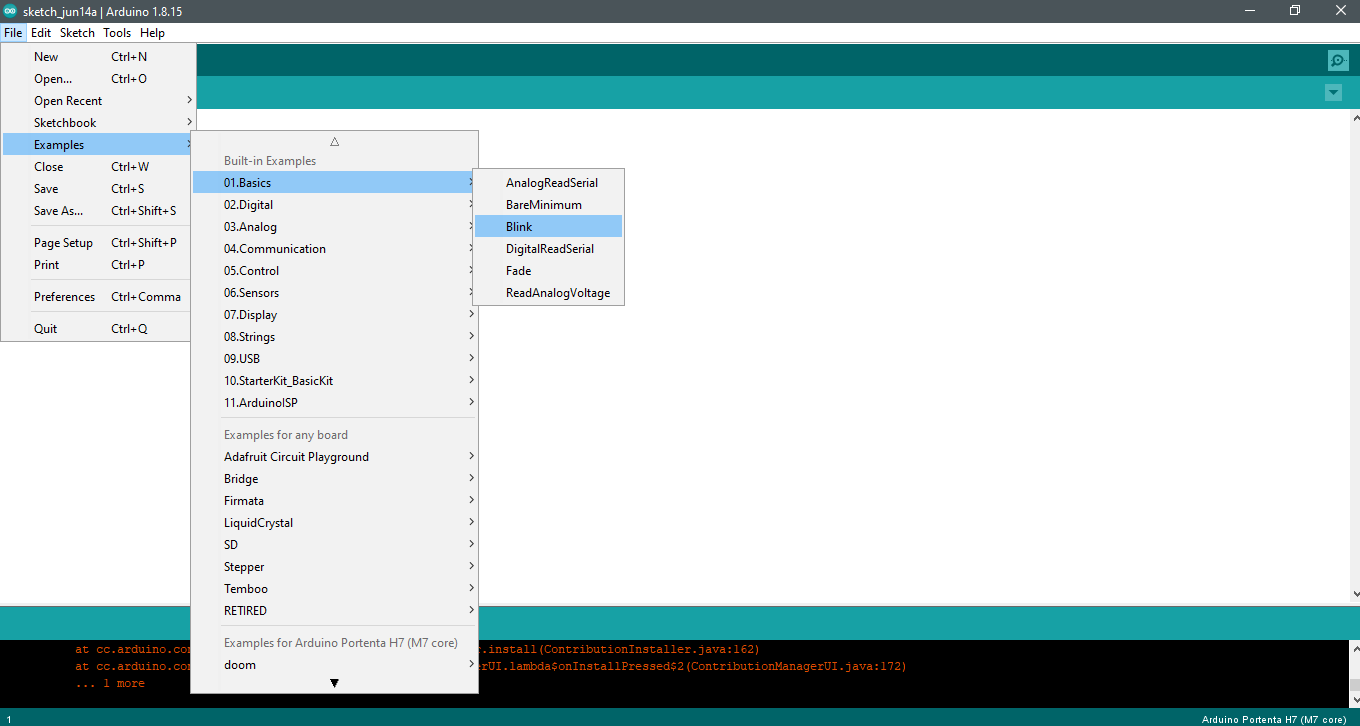
\includegraphics[width=8cm]{Images/Development Environment/Menu bar options}
	\caption{\textbf{Menu bar options.}}
	\label{fig::Menu bar options}		
\end{figure}
After the download is done, open the setup file and proceed to install.
Select all the components in the dialog box and click Next.\\

\begin{figure}[H]\centering
	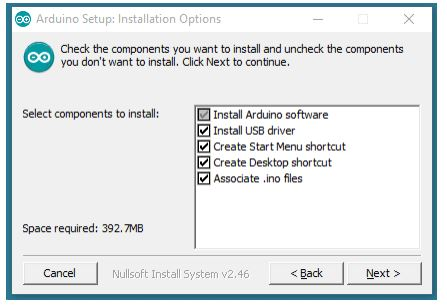
\includegraphics[width=8cm]{Images/Development Environment/Arduino Setup Installation options}
	\caption{\textbf{Arduino Setup Installation options.}}
	\label{fig:Arduino Setup Installation options}		
\end{figure}

Select the destination folder and click Install

\begin{figure}[H]\centering
	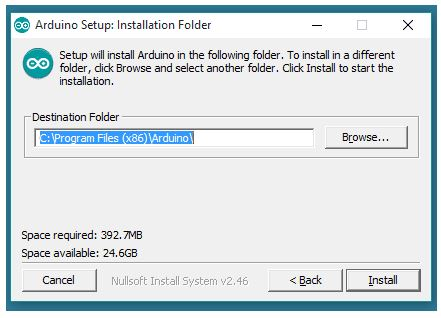
\includegraphics[width=8cm]{Images/Development Environment/Arduino Setup Installation Folder}
	\caption{\textbf{Arduino Setup Installation Folder.}}
	\label{fig:Arduino Setup Installation Folder}		
\end{figure}

Once the installation is done, open the Arduino IDE and a default sketch appears on the screen as shows.

\begin{figure}[H]\centering
	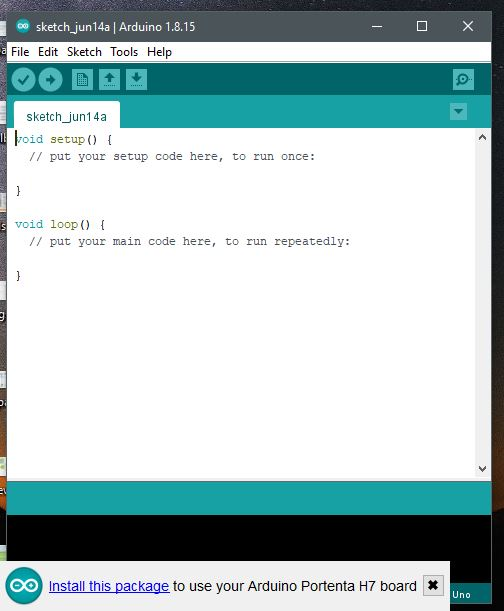
\includegraphics[width=8cm]{Images/Development Environment/Arduino Sketch}
	\caption{\textbf{Arduino Sketch.}}
	\label{fig:Arduino Sketch}		
\end{figure}


It can be seen from the above figure that the basic arduino sketch has two parts. The first part is the function \PYTHON{void setup()} which returns void and we do the intiliaztion such as the output LED color, specifying the core etc. The second part is the function \PYTHON{void loop()} where we define functions which are to be performed through out the loop. These codes are placed between paranthesis \PYTHON{$\{ \}$} and each function has a return type, here it has void return type.



\subsection{Arduino IDE on PC}
\subsubsection{Installation}
Arduino Nano 33 BLE Sense uses the Arduino software integrated development environment (IDE) for programming, which is the most widely used and common (IDE) for all arduino boards that can be run online and offline. This is a open-source Arduino Software (IDE) makes it easy to write code and upload it to the board. There are various version of software which is supported for each operating system (OS) e.g: mac, linux, and windows. Arduino community also provide us to start coding online and save our sketches in the cloud, this online arduino editor is most up-to-date version of the IDE includes all libraries and also supports new Arduino boards. For getting access to these software packages go to the following link \url{https://www.arduino.cc/en/software}  and get more up to date inforamtion, because every single day there are some updates occurs which is available on the link mention above. These software can be used with any Arduino board, the most recent offline arduino IDE 1.8.15 can be seen in Figure,\ref{fig:Arduino Creat Agent Installation}. it is also supportive for all operating systems.


\begin{figure}[H]\centering
	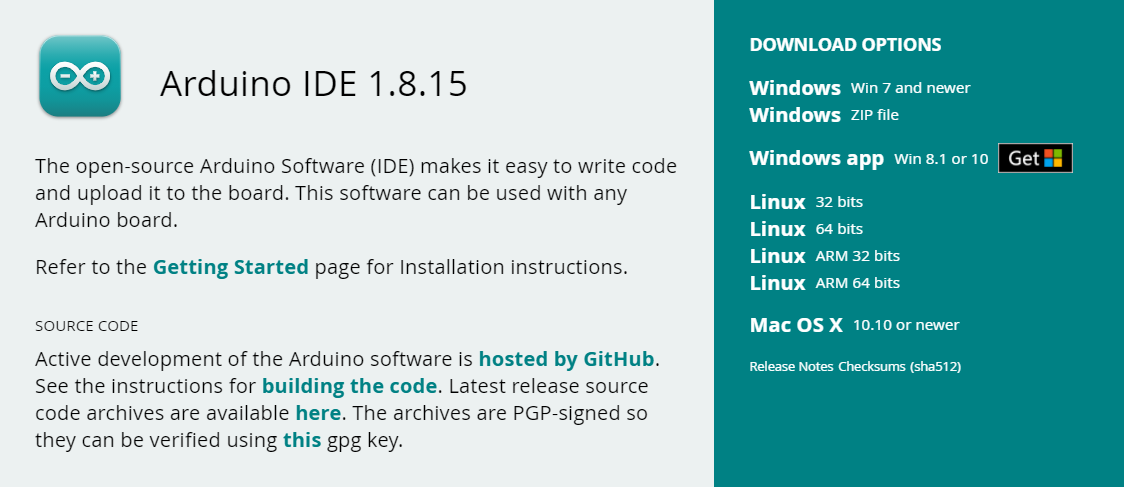
\includegraphics[width=8cm]{Images/Development Environment/Arduino Creat Agent Installation}
	\caption{\textbf{Arduino Creat Agent Installation.}}
	\label{fig:Arduino Creat Agent Installation}		
\end{figure}

\subsection{Configuration}
\subsubsection{Configuration for the Arduino Nano 33 BLE Sense}
To program the Arduino Nano 33 BLE Sense in offline state, we need to install one
of the latest arduino IDE on our desktop. After installation, for getting access to
the Arduino nano 33 ble sense board, we need to make configuration in our IDE. By
opening the IDE, go to tool which can be seen on the uper left corner in IDE, in the
tool there is an option for managed board. At this point we need to write our board
name in the search which is Arduino Nano 33 BLE Sense as shown in figure,\ref{fig:Arduino Mbed OS Nano Boards Installation}.Select
the Arduino Mbed OS Boards and install it. The Mbed OS nano board supports also
other nano family boards including Arduino nano 33 ble sense, after installing simply
connect the Arduino Nano 33 BLE Sense to the computer via USB cable.


\begin{figure}[H]\centering
	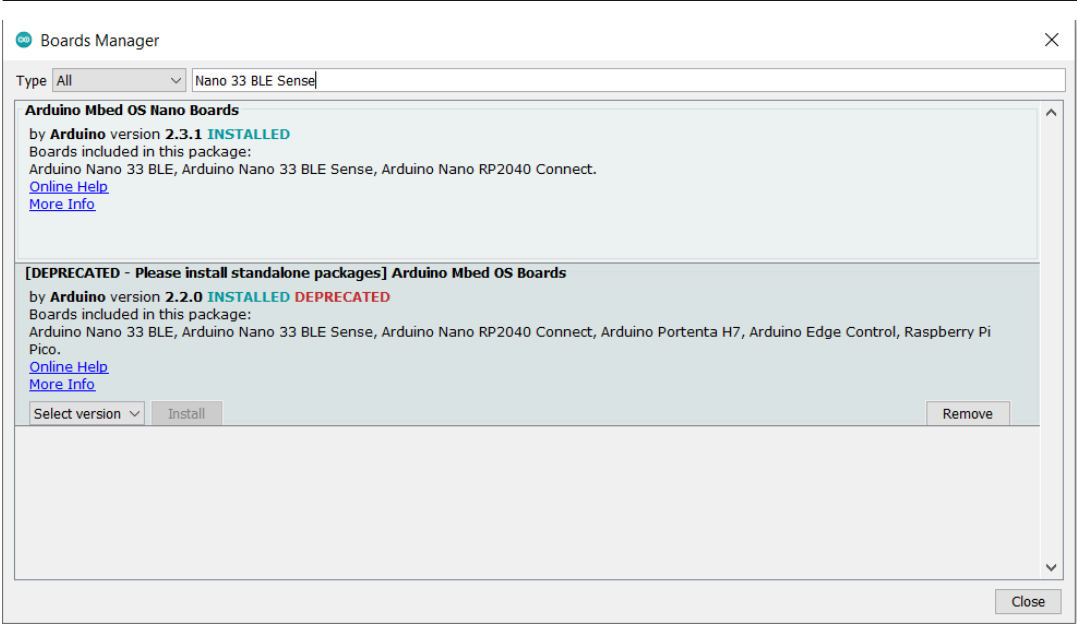
\includegraphics[width=8cm]{Images/Development Environment/Arduino Mbed OS Nano Boards Installation}
	\caption{\textbf{Arduino Mbed OS Nano Boards Installation.}}
	\label{fig:Arduino Mbed OS Nano Boards Installation}		
\end{figure}



\subsection{Setup}
There are set of examples which are build in Arduino (IDE) for the testing purpose, for checking all the configuration and setting up the board we can open one of the basic LED blink example first as shown in the figure.  \ref{fig:LED-Example Test}.



\begin{figure}[H]\centering
	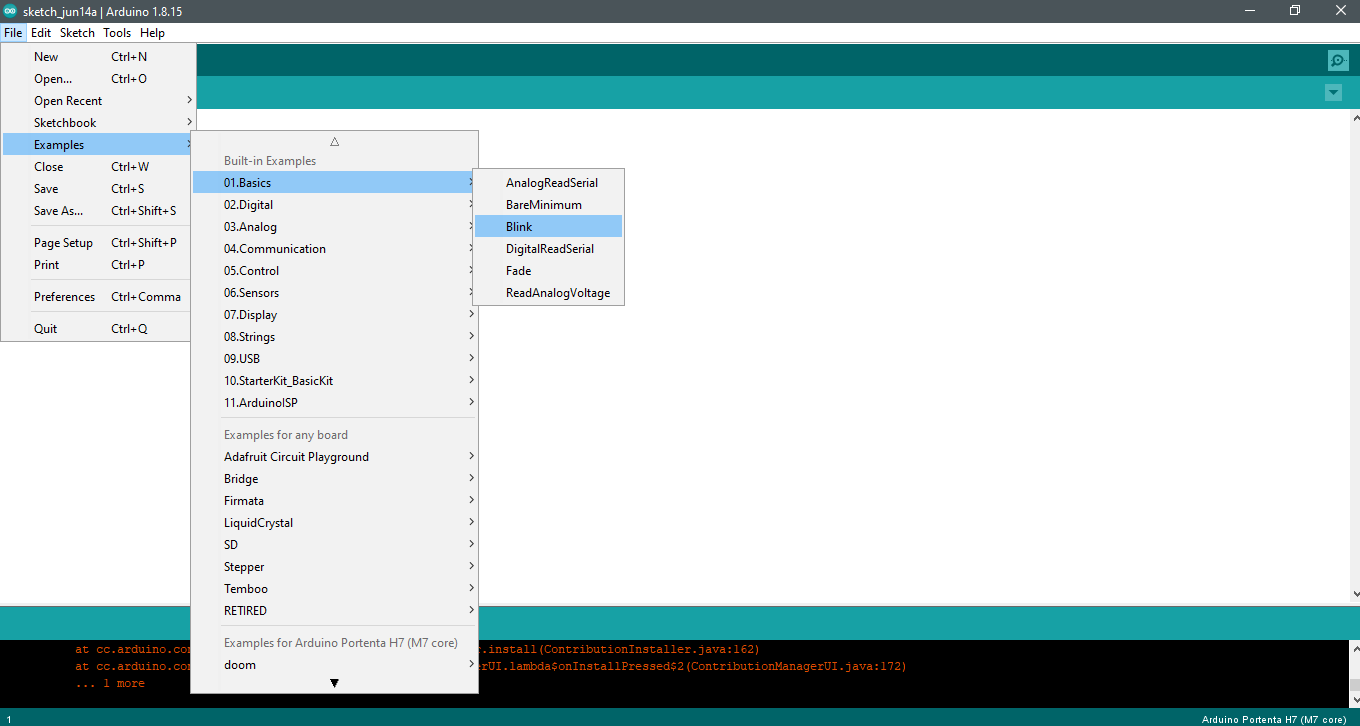
\includegraphics[width=8cm]{Images/Development Environment/Menu bar options}
	\caption{\textbf{LED-Example Test.}}
	\label{fig:LED-Example Test}		
\end{figure}
This LED-blink example support all the arduino boards, for the checking purposes just need to run this basic example on any arduino embed board and it will blink the LED on our Arduino board after pre-set miliseconds. In the same example folder, there are also number of build in usefull example written in Arduino IDE for embedded boards. These examples are very usefull for getting the basic knowledge about the board and programming.

\subsection{constraints}
There are some pre-requisite steps need to follow either we need to run the build in example or run by our own written program. By operating the Arduino board with Laptop with the help of USB connection, need to open the Arduino IDE on desktop, it appears a blank arduino environment page just a Void setup and void loop written on it. At this step we need to go to the tool-Arduino board and select the connected board which is Arduino Nano 33 Ble Sense as shown in the figure   \ref{fig:Select the Connected board -here Arduino Nano 33 BLE Sense}

\begin{figure}[H]\centering
	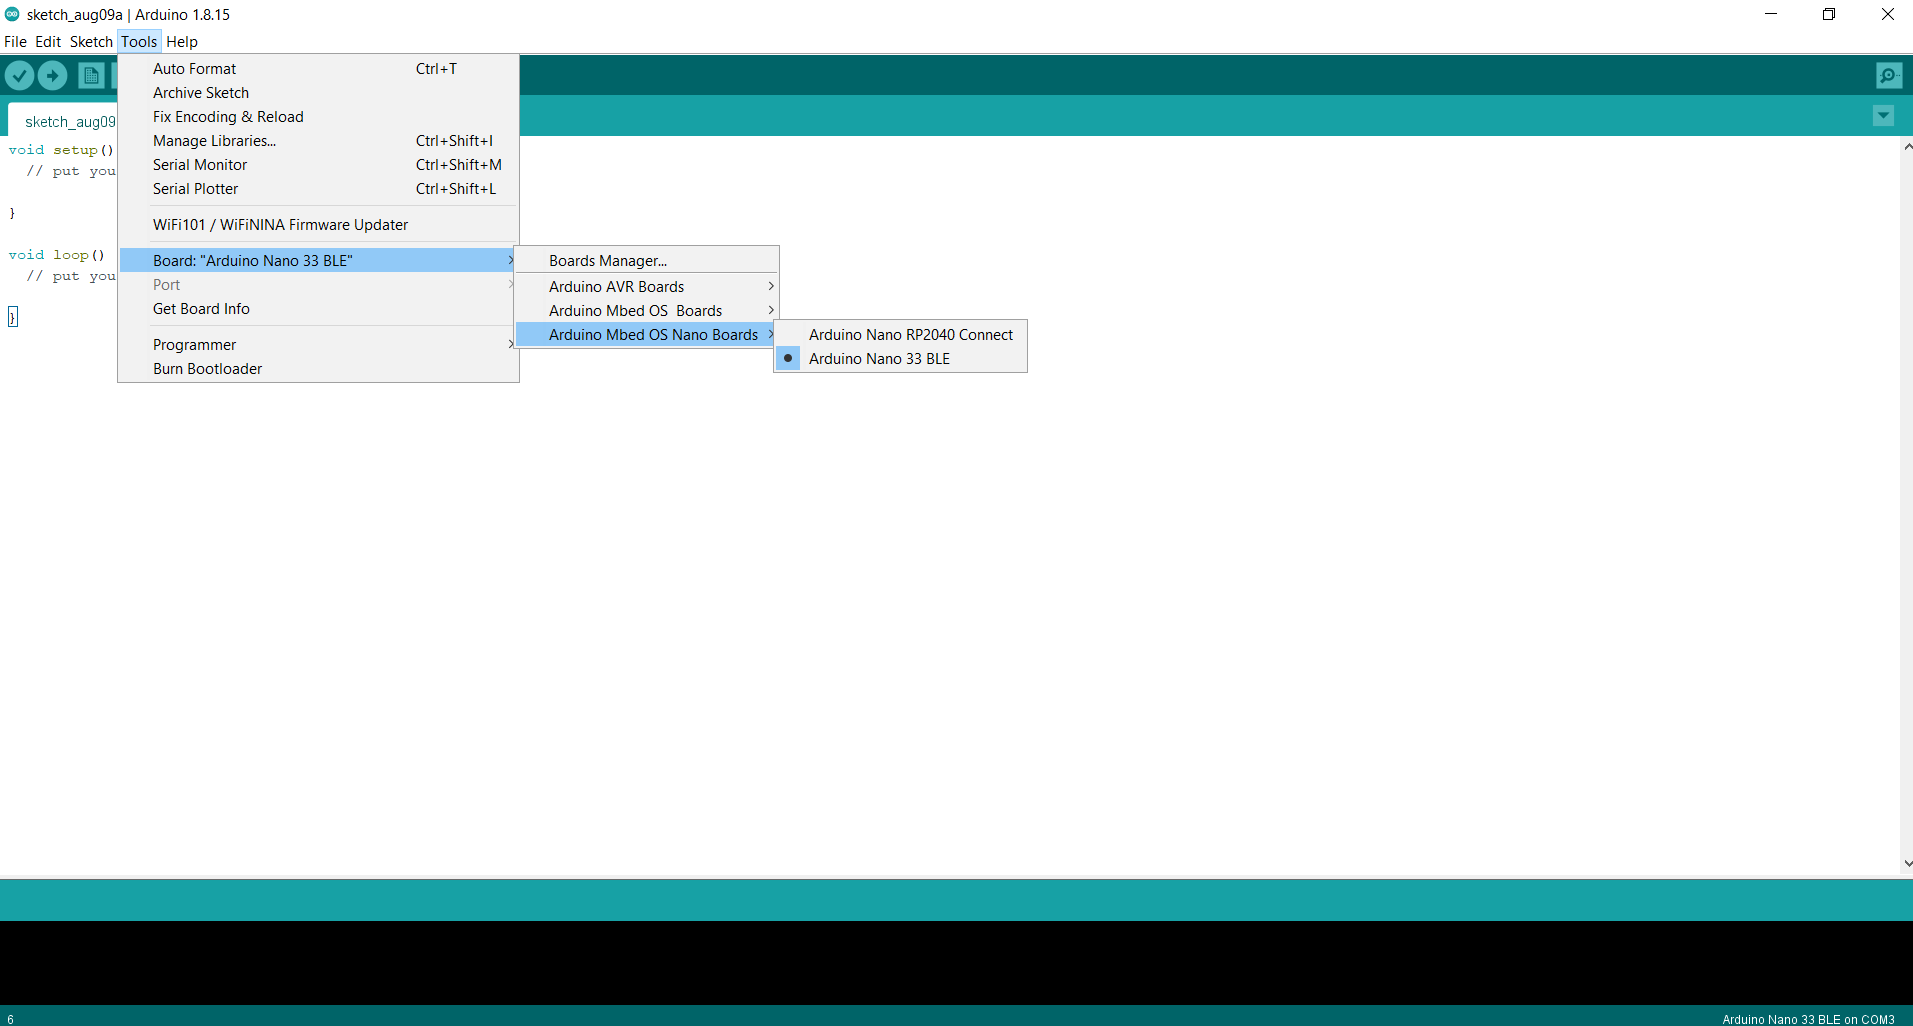
\includegraphics[width=8cm]{Images/Development Environment/Select the Connected board -here Arduino Nano 33 BLE Sense}
	\caption{\textbf{Select the Connected board -here Arduino Nano 33 BLE Sense.}}
	\label{fig:Select the Connected board -here Arduino Nano 33 BLE Sense}		
\end{figure}
\subsubsection{Select the Appropriate Port}
By selecting the Arduino nano 33 BLE sense board, next we need to check the connected port. For doing this, we need to set our arduino borad in Boot setup by clicking the white reset button on arduino as show in figure \ref{fig:Arduino Nano 33 BLE Sense Reset Button}

\begin{figure}[H]\centering
	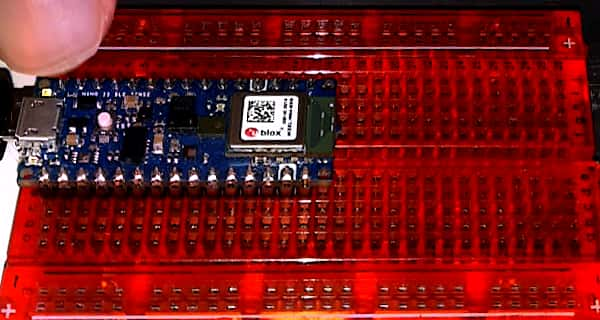
\includegraphics[width=8cm]{Images/Development Environment/Arduino Nano 33 BLE Sense Reset Button}
	\caption{\textbf{Arduino Nano 33 BLE Sense Reset Button.}}
	\label{fig:Arduino Nano 33 BLE Sense Reset Button}		
\end{figure}
By clicking the white reset button, the arduino borad will be in boot setup and make
sure to check the orange LED glows as shown in the figure\ref{fig:Arduino Nano 33 BLE Sense Orange LED Glow}
\begin{figure}[H]\centering
	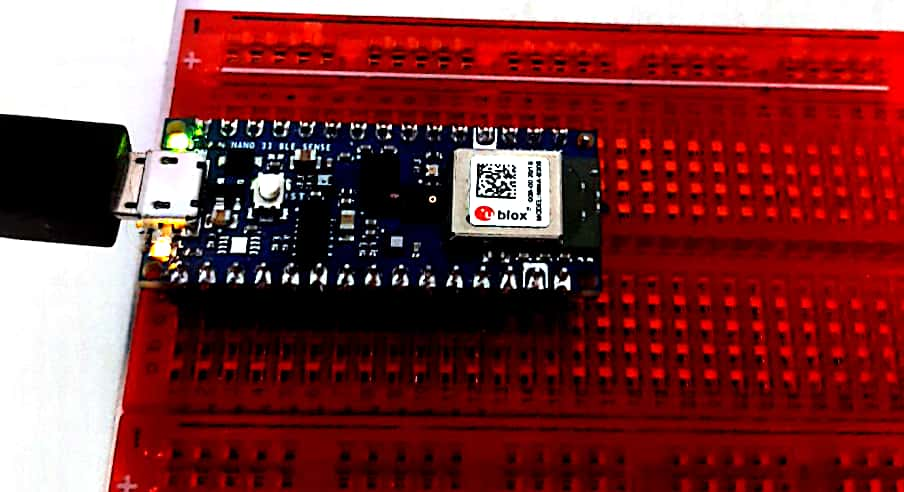
\includegraphics[width=8cm]{Images/Development Environment/Arduino Nano 33 BLE Sense Orange LED Glow}
	\caption{\textbf{Arduino Nano 33 BLE Sense Orange LED Glow.}}
	\label{fig:Arduino Nano 33 BLE Sense Orange LED Glow}		
\end{figure}
After successfully applying the above mention step, next we need to select the connected
port before upload the program. For this, go to tool select arduino port and make
sure to check it available port for uploading the program as shown in figure\ref{fig:Select Available Port for Uploading Arduino Sketch}
\begin{figure}[H]\centering
	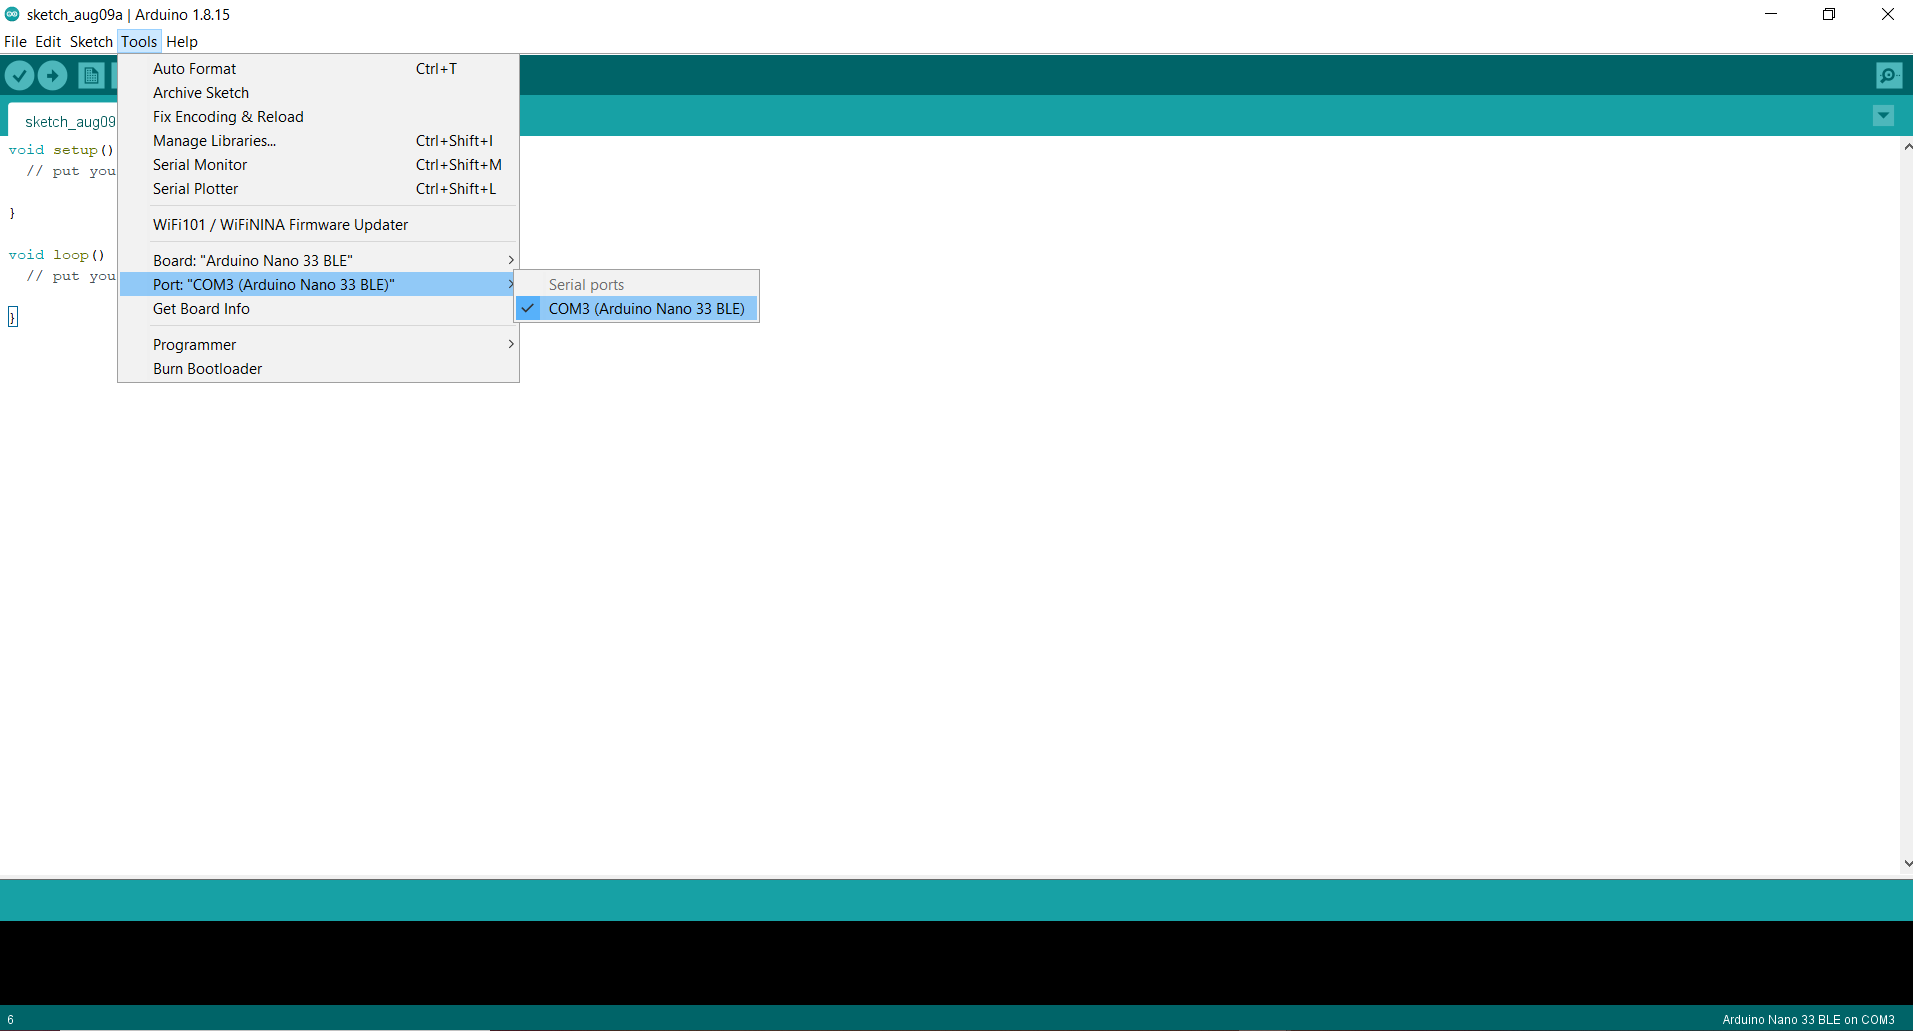
\includegraphics[width=8cm]{Images/Development Environment/Select Available Port for Uploading Arduino Sketch}
	\caption{\textbf{Select Available Port for Uploading Arduino Sketch.}}
	\label{fig:Select Available Port for Uploading Arduino Sketch}		
\end{figure}

\subsubsection{Upload Code in Arduino Board}\label{uploadcode}
By making sure to select the appropriate port, it’s time to upload the Arduino program.
There are five icons (verify, upload, new, open, save) below the file section, before
uploading the program the best practice is to verify the program first, it show us if
there are any error or warning in the program exist or not. By successfully verifying
the program we can safely upload the program by click the upload button in the top
below the file section as shown in figure.\ref{fig:Upload the Program in Arduino board}
\begin{figure}[H]\centering
	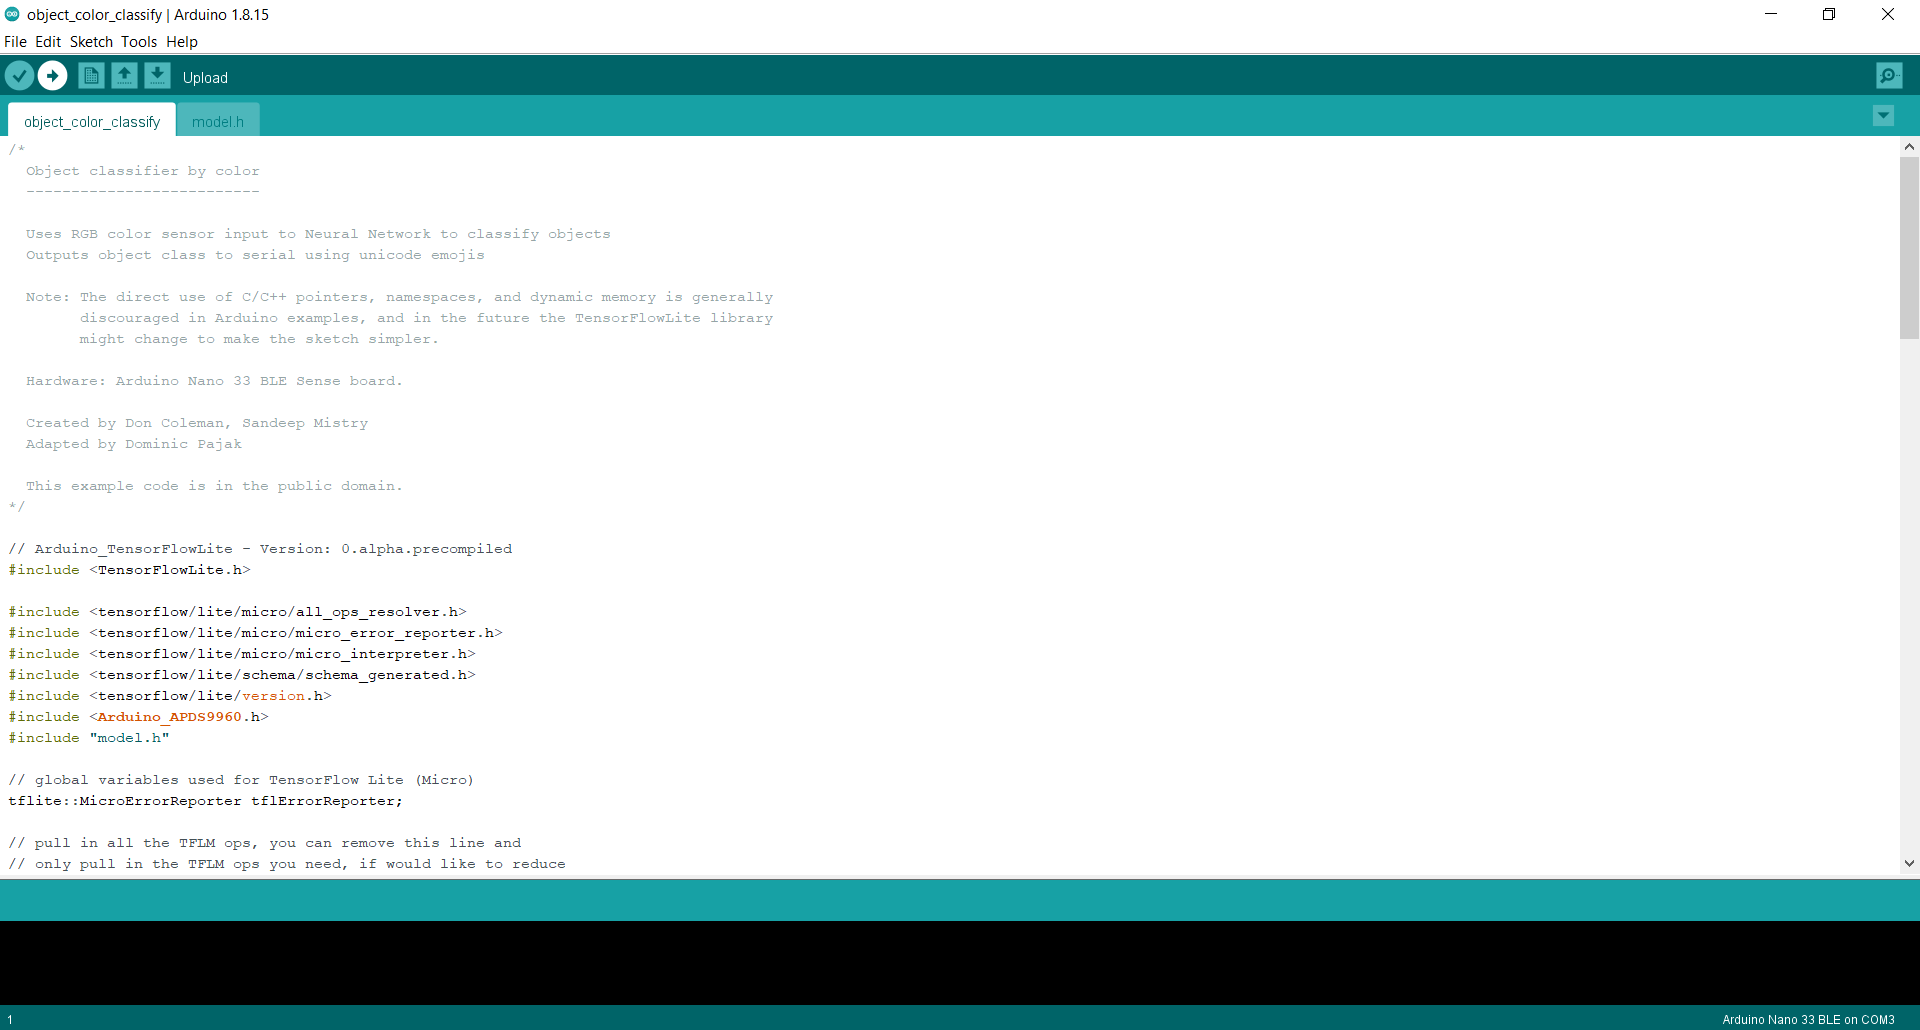
\includegraphics[width=8cm]{Images/Development Environment/Upload the Program in Arduino board}
	\caption{\textbf{Upload the Program in Arduino board.}}
	\label{fig:Upload the Program in Arduino board}		
\end{figure}
After uploading, the code will compile and if there is any issue in our program it will
pop up in the bottom black window as well.
After successfully uploading and compiling the code in Arduino board, it also require
to change the port again as we did it previously. Go to tool select arduino port and
make sure to check the port again as shown in figure\ref{fig:Setting the Port} by getting output in the
serial monitor.
\begin{figure}[H]\centering
	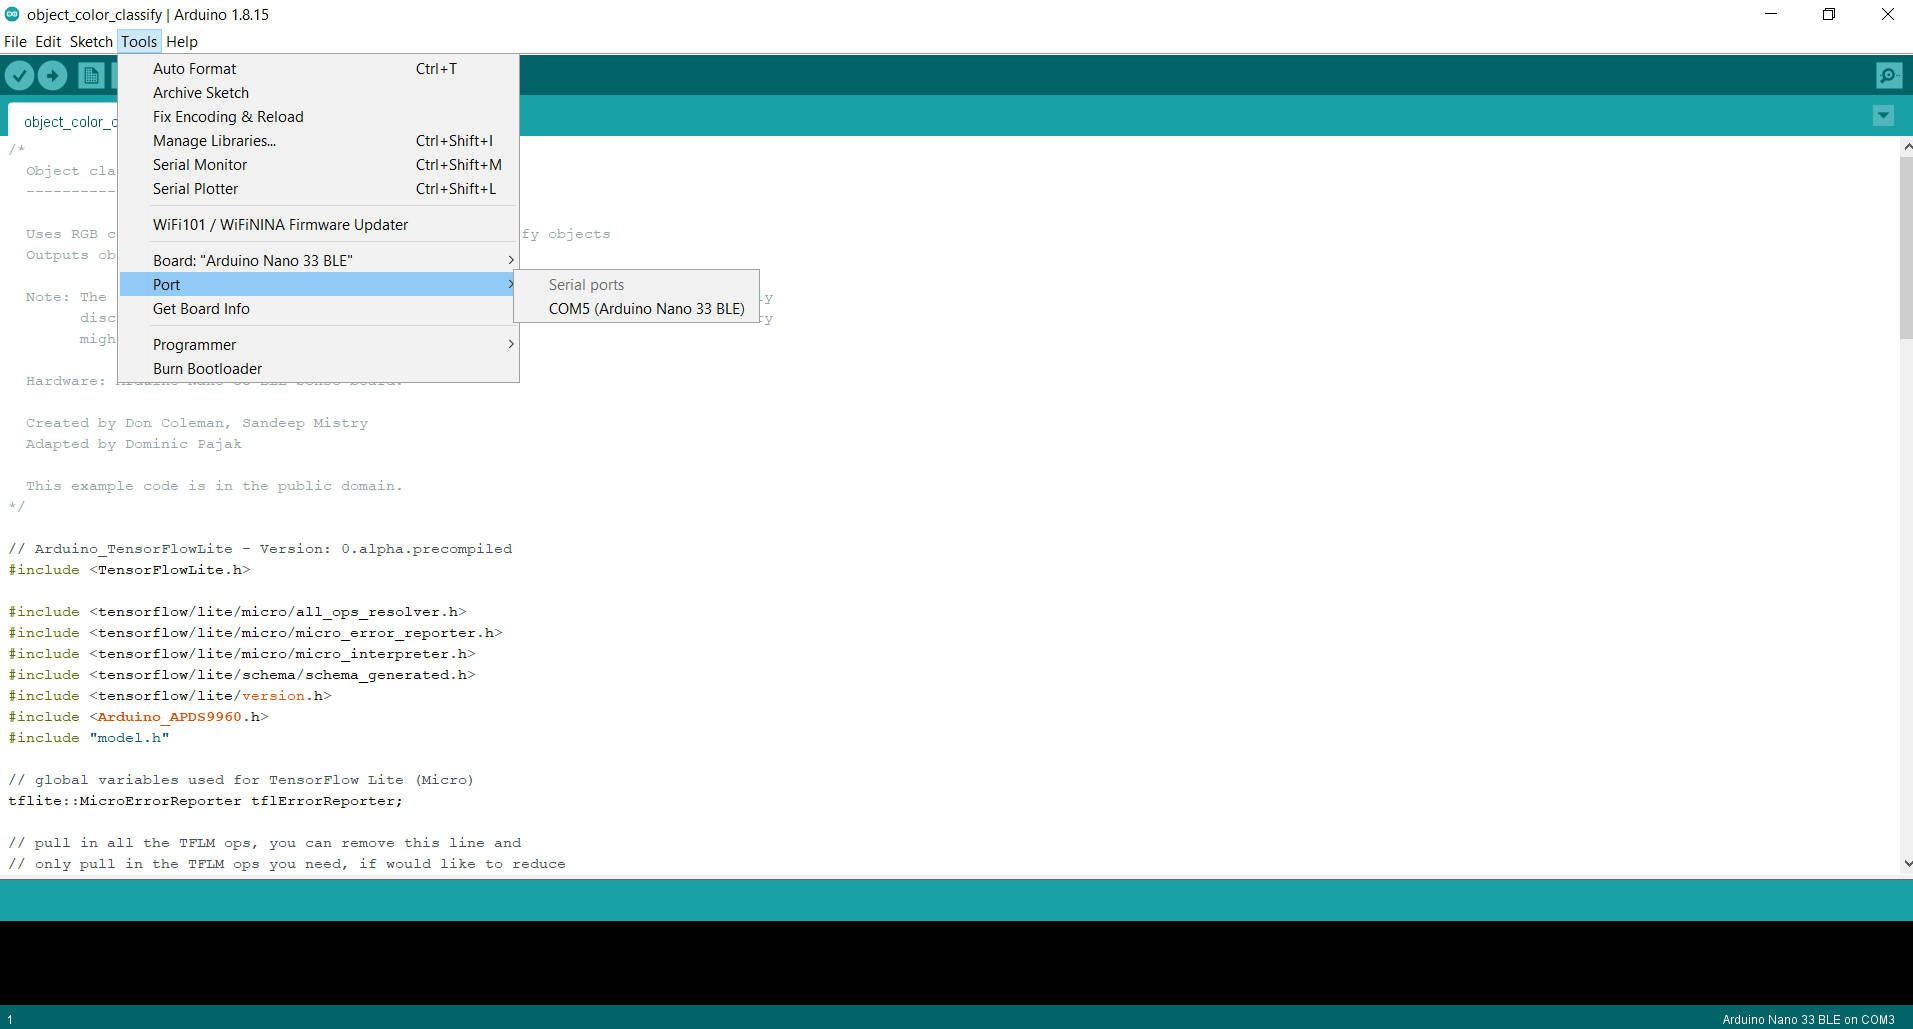
\includegraphics[width=8cm]{Images/Development Environment/Setting the Port}
	\caption{\textbf{Setting the Port.}}
	\label{fig:Setting the Port}		
\end{figure} 
\subsection{Conclusions}
\subsubsection{Output Window (Serial Monitor)}
Serial Monitor is the another window on the Arduino IDE, which shows the Input/Output of our program and results appear on it as per the required output. For getting
access to Serial monitor, we need to go extreme right in the Arduino IDE, the small
circle pop up when we reach it is the serial monitor as show in the figure.\ref{fig:Serial Monitor Icon}
\begin{figure}[H]\centering
	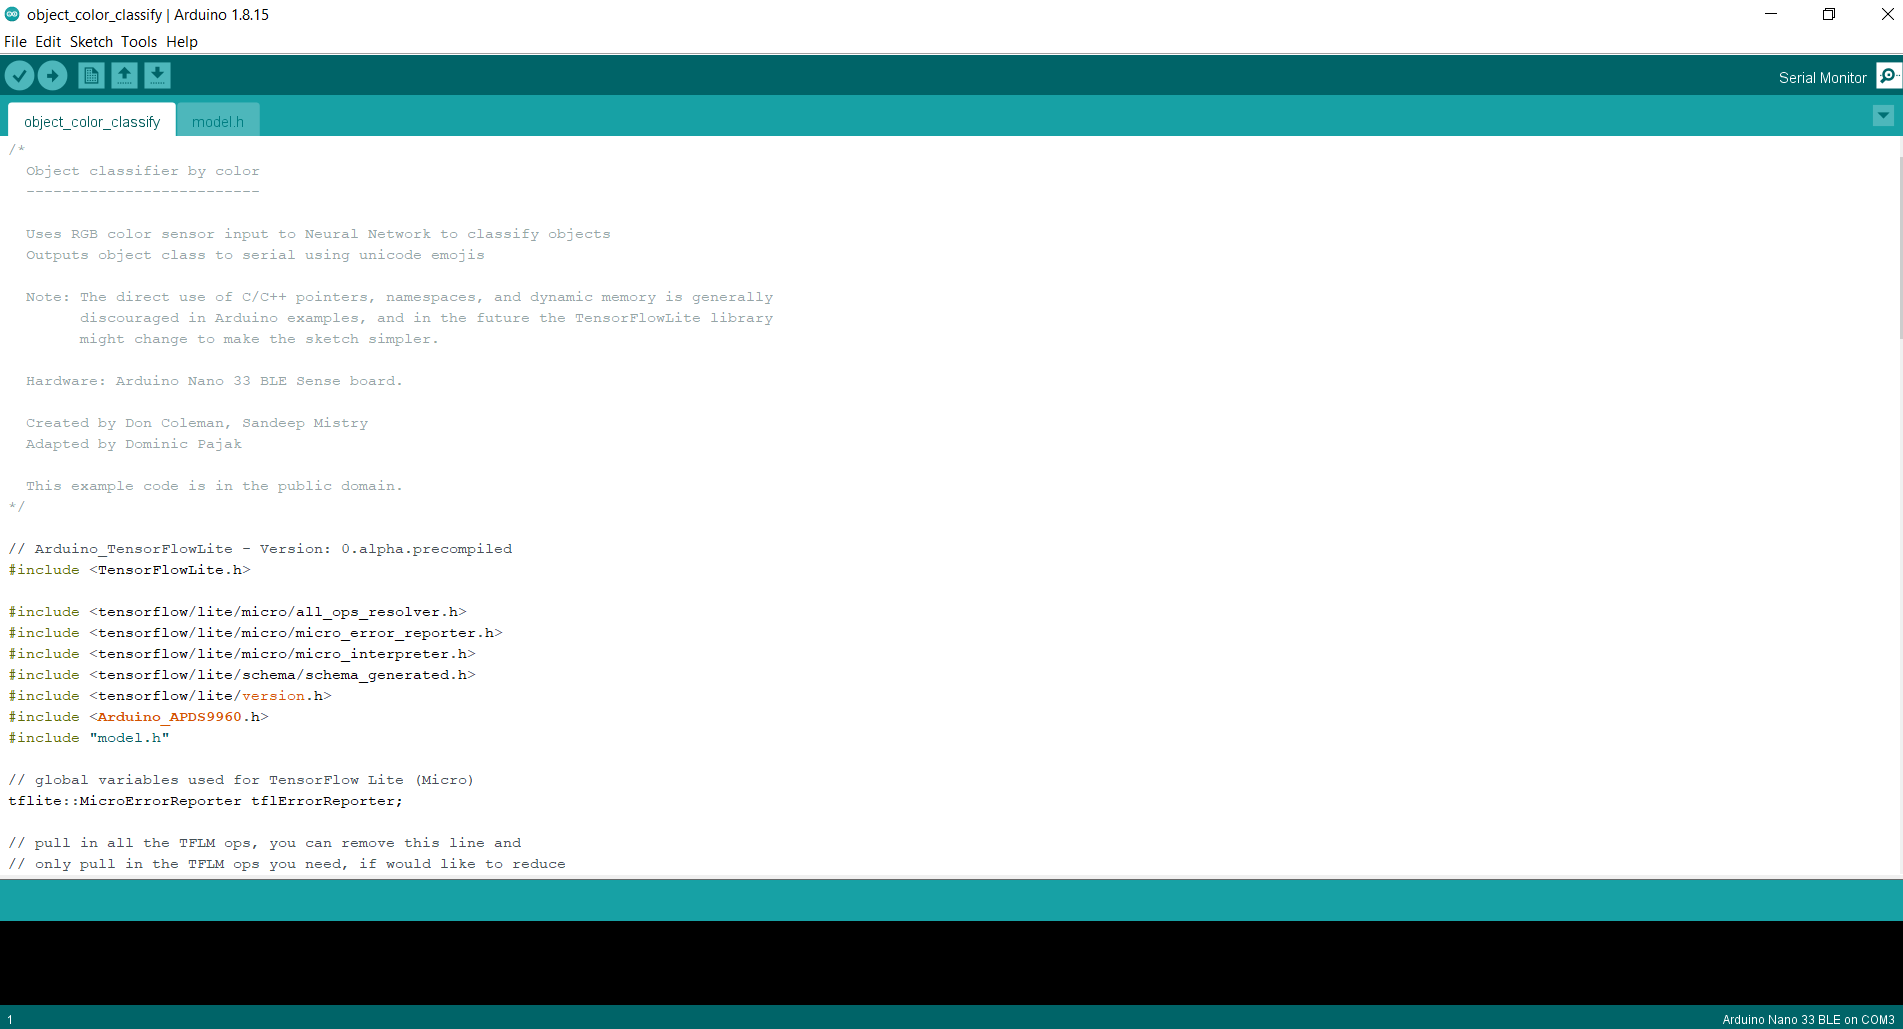
\includegraphics[width=8cm]{Images/Development Environment/Serial Monitor Icon}
	\caption{\textbf{Serial Monitor Icon.}}
	\label{fig:Serial Monitor Icon}		
\end{figure} 
The Final results, all the variables, input, sensor values are shown in the serial monitor
the (Output Window) as shown in the figure\ref{fig:Output Window} by clicking the serial monitor button.
\begin{figure}[H]\centering
	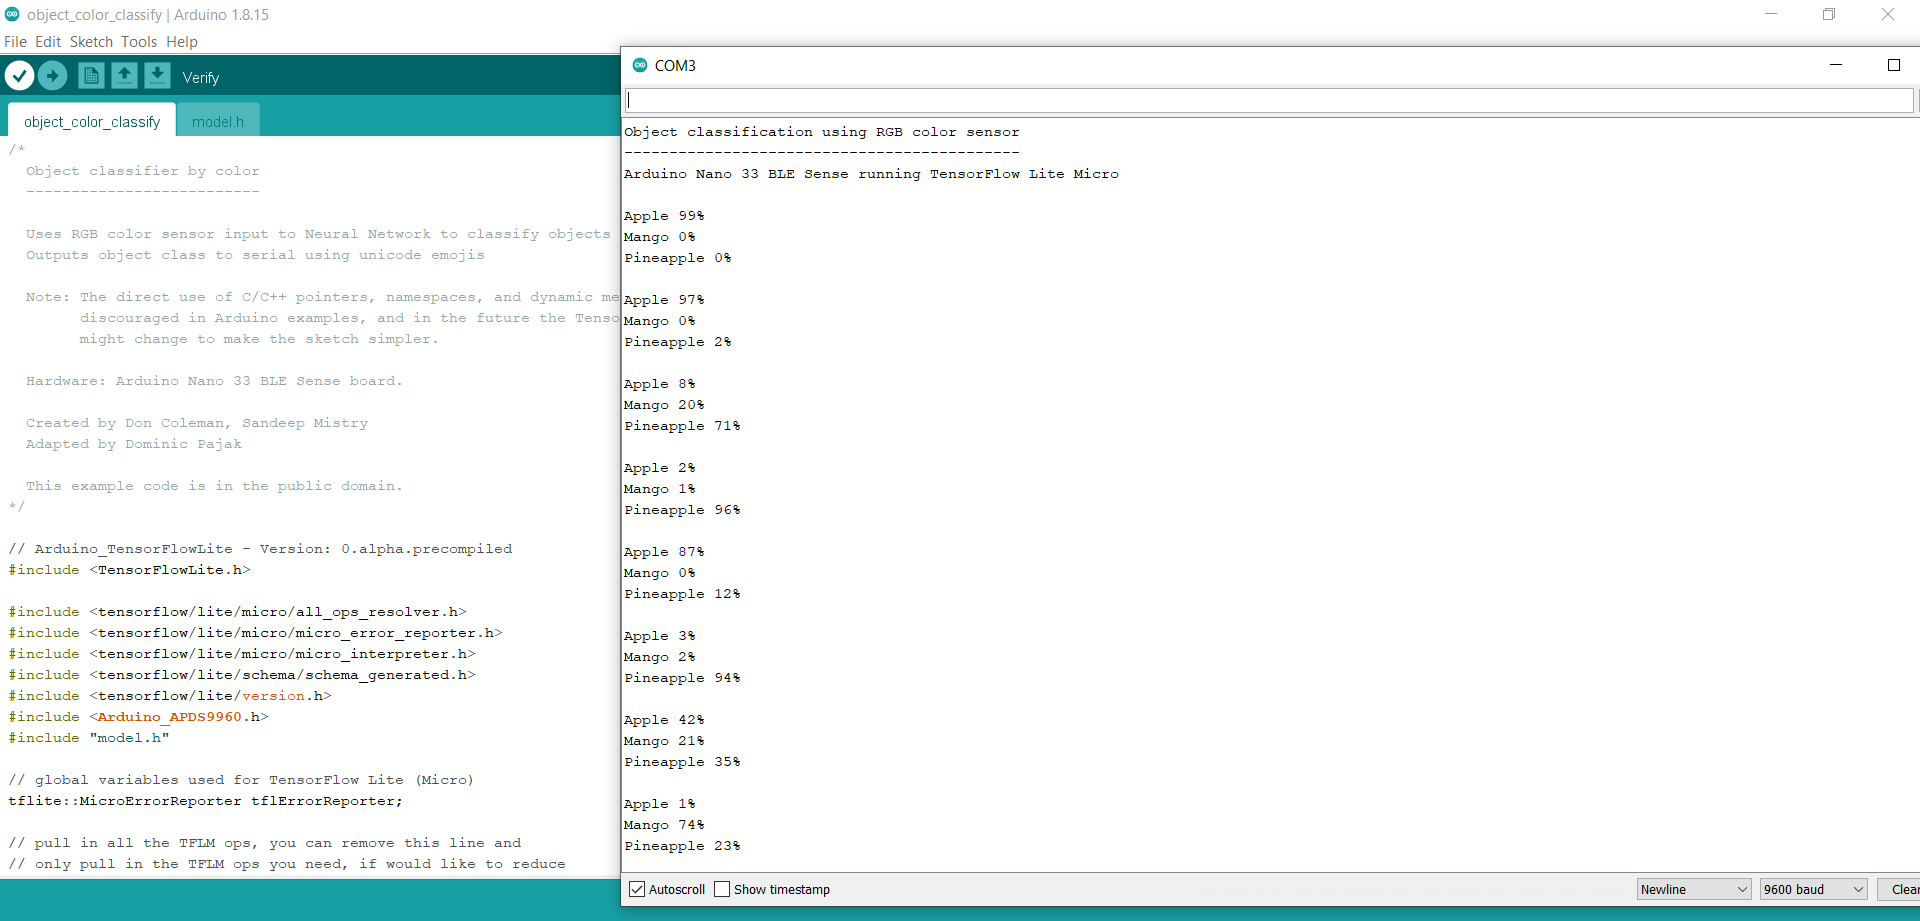
\includegraphics[width=8cm]{Images/Development Environment/Output Window}
	\caption{\textbf{Output Window.}}
	\label{fig:Output Window}		
\end{figure} 


\section{TensorFlow}
\label{TensorFlow}

\ac{tf} is an end-to-end, open-source platform popularly used for the quick implementation of machine learning algorithms. A rich ecosystem of tools, libraries, and community resources has made it extremely popular among machine learning researchers and practitioners to develop and deploy various machine learning algorithms with greater efficiency and flexibility. TensorFlow has become popular in recent times for the quick development of complex deep neural network architectures for both experimentation and developing production-ready software.\cite{TensorFlow:2023}

TensorFlow was originally developed by Google within their Machine Intelligence Research Organization to conduct various machine learning and neural networks related research. The initial version was released in 2015 under the Apache License 2.0. TensorFlow 2.0, the newest stable version, was released in 2019. TensorFlow is highly flexible. It supports a wide variety of programming languages, including Python, C++, and Java. Moreover, it can run on CPU, GPU, and TPU for a faster processing of large machine learning applications. TensorFlow is available in Linux, macOS X, and Windows platforms. It also supports TensorFlow Lite, a highly optimized lighter version of the original TensorFlow that is available on mobile computing platforms such as Android, iOS-based smartphones, and Linux-based single board computers like Raspberry Pi. TensorFlow Lite models can be further optimized using a few standard APIs to run on microcontroller units. Hence, TensorFlow is heavily used in TinyML applications. Visit the official TensorFlow website for more details. To summarize, some of the key features of TensorFlow are as follows:

\begin{itemize}
	
	\item It is open-source 
	
	\item Efficiently works with multi-dimensional data
	
	\item Provides a higher level of abstraction, which reduces the code length for the developer 
	
	\item Supports various platforms and architectures
	
	\item Highly scalable and provides greater flexibility for quick prototyping 
	
\end{itemize}

\subsection{Installation}

TensorFlow, along with all its dependencies, is already installed in Colab. So, you just need to import the libraries to write codes without any package installation. TensorFlow can be imported by typing the following command in the code cell.


\begin{lstlisting}[language=Python, caption={Import TensorFlow and Check Version}, label={code:tensorflow-version}, style=pythonstyle]
	# Import TensorFlow
	import tensorflow as tf
	
	# Check TensorFlow version
	tf._version_
\end{lstlisting}


Once TensorFlow is imported, you can check the version by typing the command \textbf{tf.\_version\_}. At the time of writing this book, the TensorFlow version in Colab is 2.12.0, which may change with time. TensorFlow 2, or TF 2, is the newest version which is significantly different compared to the previous version TF 1.x. In this book, we will use TF2 for all our programming. However, TF 2 provides a backward compatibility module to use TF 1.x. The eager execution mode of TF 2 makes it easier to create a machine learning architecture with lesser lines of code. \cite{TensorFlow:2023} 


\subsection{constraints}

Once we are done with loading and pre-processing of the data, we can define neural network architecture.
A Keras model has the following four stags:

\begin{enumerate}
	
	\item Defining the model: We define a Sequential model and add the necessary layers.
	
	\item Compiling the model: We configure the model for training by defining the loss function to be minimized, the optimizer that minimizes the loss function, and a performance metric to internally evaluate the performance. 
	
	\item Fitting the model: Here, we fit the model on the actual training data for a given number of epochs to update the training parameters. We will get the model at the end of training.
	
	\item Evaluation: Once you have the model, you can evaluate on unseen test data
	
\end{enumerate}


\subsection{Conclusions}

One of the biggest benefits of using TensorFlow is the level of abstraction. It takes care of the major details of most of the underlying algorithms in a machine learning or a deep learning application, for example, backpropagation. Hence, writing programs in TensorFlow is super easy as you mostly need to focus on your application logic. TensorFlow applications can run on almost any target environment, such as local desktops, remote servers running Windows, Linux, macOS X, smartphone devices running Android and iOS, or Linux-based single board computers. TensorFlow contains additional libraries to convert a machine learning model into C++ equivalent libraries to run on selected microcontrollers. Hence, you can use TensorFlow to create your TinyML applications. Throughout this book, we will primarily use Keras to implement the machine learning models. Keras is a high-level set of Python \ac{api} in TensorFlow, which is popularly used in the rapid prototyping of various neural network models. Fortunately, both TensorFlow and Keras are readily available in Colab. So, you can easily start writing your program in Colab without installing any extra libraries. In this chapter, we will primarily focus on creating end-to-end neural network models using TensorFlow. The later chapters will focus on optimizing the neural networks to create deployable TinyML applications.


%\section{Conclusion}
%
%Python is a very popular programming language in machine learning for researchers and also for developing production-ready software. A good understanding of Python is a prerequisite to fully understand the rest of the topics covered in the book. This chapter has been designed as a crash course to brush up on your Python programming knowledge before moving to the more complex part of programming in deep learning and TinyML applications. We assume that the readers have some fundamental knowledge of Python programming. Those who require an in-depth knowledge of Python and its various libraries are strongly encouraged to read the various resources available in print and also in digital mediums. The readers should try to execute the examples covered in this book at their end and are also strongly encouraged to modify, tweak, and extend them to gain more confidence in writing their own codes independently.

%\section{Further reading}
%
%\begin{enumerate}
%	
%	\item \textbf{Beazley, David, and Brian K. Jones. Python cookbook: Recipes for mastering Python 3. "O'Reilly Media, Inc.", 2013.}
%	
%	This book provides a collection of practical and diverse Python recipes for mastering the language. It covers a wide range of topics and scenarios, offering solutions and insights that help developers become more proficient in Python programming.
%	
%	\item \textbf{Pajankar, Ashwin. "Introduction to Python." In Python Unit Test Automation, pp. 1-17. Apress, Berkeley, CA, 2017.}
%	
%	Introducing Python through the lens of unit testing, this book explains the fundamentals of Python and how to apply them to automate unit testing. It's a practical guide that combines Python programming with testing practices for software quality assurance.
%	
%	\item \textbf{Cutler, Josh, and Matt Dickenson. "Introduction to Machine Learning with Python." In Computational Frameworks for Political and Social Research with Python, pp. 129-142. Springer, Cham, 2020.}
%	
%	Embedded within a broader context of computational frameworks for social and political research, this book offers an introduction to machine learning concepts using Python. It explores the application of machine learning techniques in the realm of social and political research.
%	
%	\item \textbf{Joshi, Prateek. Artificial intelligence with Python. Packt Publishing Ltd, 2017.}
%	
%	Focused on artificial intelligence, this book provides insights into various AI techniques using Python. It covers topics like machine learning, natural language processing, and neural networks, guiding readers through the implementation of AI models.
%	
%	\item \textbf{Campesato, Oswald. TensorFlow 2 Pocket Primer. Stylus Publishing, LLC, 2019.}
%	
%	This concise primer delves into TensorFlow 2, a popular deep learning framework. It offers a quick reference for readers to understand and work with TensorFlow 2, covering essential concepts and techniques.
%	
%	\item \textbf{Singh, Pramod, and Avinash Manure. Learn TensorFlow 2.0: Implement Machine Learning and Deep Learning Models with Python. Apress, 2019.}
%	
%	Centered around TensorFlow 2.0, this book provides practical guidance on implementing machine learning and deep learning models using Python. It offers step-by-step examples and insights into various aspects of deep learning.
%	
%\end{enumerate}
%

\section{TensorFlow Lite}
To meet these lower size requirements for mobile platforms, in 2017 Google started a companion project to mainline TensorFlow called TensorFlow Lite. This library is aimed at running neural network models efficiently and easily on mobile devices. To reduce the size and complexity of the framework, it drops features that are less cons mon on these platforms. For example, it doesn't support training, just running infer ence on models that were previously trained on a cloud platform. It also doesn't support the full range of data types (such as double) available in mainline Tensor Flow Additionally, some less-used operations aren't present, like tf.depth\_to\_space You can find the latest compatibility information on the TensorFlow website.

In return for these trade-offs, TensorFlow Lite can fit within just a few hundred kilo- bytes, making it much easier to fit into a size-constrained application. It also has highly optimized libraries for Arm Cortex-A-series CPUs, along with support for Android's Neural Network API for accelerators, and GPUs through OpenGL Another key advantage is that it has good support for 8-bit quantization of networks Because a model might have millions of parameters, the 75\% size reduction from 32- bit floats to 8-bit integers alone makes it worthwhile, but there are also specialized code paths that allow inference to run much faster on the smaller data type.\cite{TensorFlow:2023}



\subsection{Installation}

\begin{lstlisting}[language=Python, caption={Load and Run TensorFlow Lite Model}, label={code:tflite-inference}, style=pythonstyle]
	import tensorflow as tf
	import numpy as np
	
	# Load the TensorFlow Lite model.
	interpreter = tf.lite.Interpreter(model_path="model.tflite")
	interpreter.allocate_tensors()
	
	# Get the input and output tensors.
	input_details = interpreter.get_input_details()
	output_details = interpreter.get_output_details()
	
	# Create some input data.
	input_data = np.array([[1.0, 2.0, 3.0]])
	
	# Set the input tensor.
	interpreter.set_tensor(input_details[0]["index"], input_data)
	
	# Perform inference.
	interpreter.invoke()
	
	# Get the output tensor.
	output_data = interpreter.get_tensor(output_details[0]["index"])
	
	# Print the output.
	print(output_data)
\end{lstlisting}


\subsection{constraints}

TensorFlow Lite for Microcontrollers is designed for the specific constraints of microcontroller development.\cite{TensorFlow:2023} If you are working on more powerful devices (for example, an embedded Linux device like the Raspberry Pi), the standard TensorFlow Lite framework might be easier to integrate The following limitations should be considered:

\begin{itemize}
	
	\item Support for a limited subset of TensorFlow operations.
	
	\item Support for a limited set of devices.
	
	\item Low-level C++ API requiring manual memory management.
	
	\item On device training is not supported
	
\end{itemize}

\subsection{Conclusions}
TensorFlow Lite is a lightweight version of TensorFlow, designed specifically for mobile and embedded devices. In the TinyML magic wand
project using Arduino Nano, TensorFlow Lite is used to run a pre-trained
machine learning model on the Arduino Nano board.
The magic wand project involves using a gesture recognition model
to detect different hand movements and control a small toy wand. The
Arduino Nano board is used to collect sensor data from an accelerometer
and gyro sensor, which is then fed into the machine learning model running
on the board. The model uses TensorFlow Lite to make predictions based
on the sensor data and determine what hand gesture is being made. Based
on the prediction, the wand can be controlled to perform different actions.
The use of TensorFlow Lite in this project allows the machine learning
model to run efficiently on the limited resources of the Arduino Nano
board. By using a lightweight model and optimizing the code for the
microcontroller architecture, it is possible to perform gesture recognition
on a low-power, low-cost device like the Arduino Nano. This makes the
project more accessible and affordable for hobbyists and students who
want to experiment with TinyML applications.\cite{Magicwand:2024}



\section{TensorFlow Lite for Microcontrollers}

\subsection{Introduction}

TensorFlow Lite has been widely adopted by mobile developers, but its engineering trade-offs didn't meet the requirements of all platforms. The team noticed that there were a lot of Google and external products that could benefit from machine learning being build on embedded platforms, on which the existing TensorFlow Lite library wouldn't fit. Again, the biggest constraint was binary size. For these environments even a few hundred kilobytes was too large; they needed something that would fit within 20 KB or less. A lot of the dependencies that mobile developers take for gran- ted. like the C Standard Library, weren't present either, so no code that relied on these libraries could be used. A lot of the requirements were very similar, though. Inference was the primary use case, quantized networks were important for performance, and having a code base that was simple enough for developers to explore and modify was a priority.\cite{TensorFlow:2023}

\subsection{Work Flow}

\begin{enumerate}
	
	\item Train a model:
	
	\begin{itemize}
		
		\item Generate a small TensorFlow model that can fit your target device and contains supported operations.
		
		\item Convert to a TensorFlow Lite model using the TensorFlow Lite converter.
		
		\item Convert to a C byte array using standard tools to store it in a read-only program memory on device.
		
	\end{itemize}
	
	\item Run inference on device using the C++ library and process the results.
	
\end{enumerate}
\subsection{Installation}

\begin{lstlisting}[language=C++, caption={Run Inference with TensorFlow Lite Micro}, label={code:tflite-micro-inference}, style=bashstyle]
	#include "model.h"
	#include "tensorflow/lite/micro/kernels/micro_ops.h"
	#include "tensorflow/lite/micro/micro_error_reporter.h"
	#include "tensorflow/lite/micro/micro_interpreter.h"
	#include "tensorflow/lite/version.h"
	
	// Create an instance of the error reporter
	static tflite::MicroErrorReporter micro_error_reporter;
	
	// Define the tensor arena
	static constexpr int kTensorArenaSize = 2 * 1024;
	static uint8_t tensor_arena[kTensorArenaSize];
	
	// Create an instance of the interpreter
	static tflite::MicroInterpreter static_interpreter(
	model, tflite::MicroOpResolver::GetDefault(), tensor_arena,
	kTensorArenaSize, &micro_error_reporter);
	
	// Allocate memory for the input and output tensors
	TfLiteTensor* input = static_interpreter.input(0);
	TfLiteTensor* output = static_interpreter.output(0);
	
	// Perform inference
	static_interpreter.Invoke();
	
	// Print the output
	for (int i = 0; i < output->bytes; i++) {
		printf("%f ", output->data.f[i]);
	}
\end{lstlisting}


\subsection{constraints}

Running in embedded environments imposed a lot of constraints on how the code could be written, so it identified some key requirements for the library:

\begin{enumerate}
	
	\item \textbf{No operating system dependencies}
	
	A machine learning model is fundamentally a mathematical black box where numbers are fed in, and numbers are returned as the results. Access to the rest of the system shouldn't be necessary to perform these operations, so it's possible to write a machine learning framework without calls to the underlying operating system. Some of the targeted platforms don't have an OS at all, and avoiding any references to files or devices in the basic code made it possible to port to those chips.\cite{War:2020}
	
	\item \textbf{No standard Cor C++ library dependencies at linker time }
	
	This is a bit subtler than the OS requirement, but the team was aiming to deploy on devices that might have only a few tens of kilobytes of memory to store a pro- gram, so the binary size was very important. Even apparently simple functions like sprintf() can easily take up 20 KB by themselves, so the team aimed to avoid anything that had to be pulled in from the library archives that hold the implementations of the C and C++ standard libraries. This was tricky because there's no well-defined boundary between header-only dependencies (like stdint.h, which holds the sizes of data types) and linker-time parts of the standard libraries (such as many string functions or sprintf().
	
	\item \textbf{No floating point hardware expected }
	
	Many embedded platforms don't have support for floating-point arithmetic in hardware, so the code had to avoid any performance-critical uses of floats. This meant focusing on models with 8-bit integer parameters, and using 8-bit arith metic within operations (though for compatibility the framework also supports float ops if they're needed). \cite{Ard:2021}
	
	\item \textbf{No dynamic memory allocation}
	
	A lot of applications using microcontrollers need to run continuously for months or years. If the main loop of a program is allocating and deallocating memory using malloc()/new and free()/delete, it's very difficult to guarantee that the heap won't eventually end up in a fragmented state, causing an allocation failure and a crash. There's also very little memory available on most embedded systems, so upfront planning of this limited resource is more important than on other platforms, and without an OS there might not even be a heap and allocation rou- tines. This means that embedded applications often avoid using dynamic memory allocation entirely. Because the library was designed to be used by those applications, it needed do the same. 
	
	In practice the framework asks the calling application to pass in a small, fixed-size arena that the framework can use for temporary allocations (like activation buffers) at initialization time. If the arena is too small, the library will return an error immediately and the client will need to recompile with a larger arena. Otherwise, the calls to perform inference happen with no further memory allocations, so they can be made repeatedly with no risk of heap fragmentation or memory errors.\cite{War:2020}
	
\end{enumerate}

\subsection{Conclusions}
In the TinyML magic wand project using Arduino Nano, TensorFlow Lite Micro is used to run a machine learning model on the Arduino Nano board to recognize gestures made with the wand. The model is trained to recognize a specific set of gestures (e.g., waving the wand up and down,
left and right) and can trigger different actions based on the recognized
gesture (e.g., turn on/off lights, play music).
Using TensorFlow Lite Micro on the Arduino Nano enables the wand
to perform gesture recognition locally on the device, without the need
for an internet connection or a more powerful computer. This makes the
wand more portable and flexible, and can be used in a wider range of
environments and applications.
Overall, TensorFlow Lite Micro enables the development of TinyML
(Tiny Machine Learning) applications that run on microcontrollers and other embedded devices, making it possible to bring machine learning
capabilities to a wide range of IoT and edge devices.\cite{Gomez:2012}

Our application will be deployed on Arduino Nano 33 BLE Sense, which is a recommended microcontroller board for TinyML applications. The application we are going to implement is fairly simple. The microcontroller will read the linearly varying electrical voltage provided by an external potentiometer as its input, convert the voltage values as per a halfwave sinusoid function using a simple neural network, and controls the brightness of an LED accordingly. Remember, due to its resource constraints, you cannot even train a small neural network on a microcontroller. We will train the neural network in Colab using TensorFlow, The model will be converted into a TFLite model. This part of the project will be implemented in Python. We will then convert the model into an equivalent C/C++ library for microcontrollers. Next, we will write an inference application for Arduino using a programming language that is very similar to C/C++. 

\section{Python}
The Arduino IDE is written only in C++ language and is not supported the other programming languages. Some of the Module I used specially for executing the Gesture detection part of this project is only support python language e.g., MediaPipe and OpenCV. MediaPipe and OpenCV module are the most important part for gesture detection, for detecting the landmarks on hand the supported function is written in python. Without the MediaPipe Module, the hand landmarks technique is not possible to implement. At the moment, there is no such module or library who can support directly MediaPipe Module in Arduino IDE and C++, because MediaPipe Module is written in python.\cite{Alk:2019}
\subsection{Installation}
\label{Python}
\begin{lstlisting}[language=Python, caption={Load and Run TensorFlow Lite Model}, label={code:tflite-inference-python}, style=pythonstyle]
	import tensorflow as tf
	import numpy as np
	
	# Load the TensorFlow Lite model.
	interpreter = tf.lite.Interpreter(model_path="model.tflite")
	interpreter.allocate_tensors()
	
	# Get the input and output tensors.
	input_details = interpreter.get_input_details()
	output_details = interpreter.get_output_details()
	
	# Create some input data.
	input_data = np.array([[1.0, 2.0, 3.0]])
	
	# Set the input tensor.
	interpreter.set_tensor(input_details[0]["index"], input_data)
	
	# Perform inference.
	interpreter.invoke()
	
	# Get the output tensor.
	output_data = interpreter.get_tensor(output_details[0]["index"])
	
	# Print the output.
	print(output_data)
\end{lstlisting}

\subsection{constraints}
Python, although versatile, has constraints in the context of the magic wand project with Arduino Nano 33 BLE. Real-time operations pose a challenge due to Python's lack of native support, potentially affecting precise timing for gesture recognition. Additionally, Python's interpreted nature may result in slower execution, impacting sensor data processing and model inference speed. Memory usage can be a concern on resource-constrained microcontrollers, like Arduino Nano. While Python is not inherently optimized for the lightweight requirements of such devices, developers can mitigate these constraints by employing efficient coding practices and considering alternatives for critical real-time tasks.


\subsection{Conclusion}
The use of Python in the software aspect of the magic wand project enhances flexibility, allowing for efficient data processing, machine learning model training, and seamless communication with the Arduino Nano 33 BLE.


\section{PyCharm}
\label{Pycharm}
PyCharm, a robust Python integrated development environment (IDE), plays a pivotal role in the software development process for the magic wand project with Arduino Nano. Leveraging PyCharm's advanced code editing and navigation features, the development team benefits from an efficient and organized coding experience. The IDE's support for project management, version control integration with Git, and seamless debugging and profiling tools contribute to a streamlined development workflow. PyCharm's capabilities extend to virtual environment support, ensuring effective dependency management for the machine learning aspects of the project. Additionally, PyCharm facilitates integration with continuous integration (CI) systems, enabling automated testing and build processes. Overall, PyCharm proves indispensable in enhancing code quality, collaboration, and the overall efficiency of the machine learning software development on the Arduino Nano platform.\cite{Learn:2021}
\subsection{Setup}
To install PyCharm, begin by visiting the official PyCharm website and downloading the appropriate version for your needs—Community (free) or Professional (paid). Run the installer, typically an executable file on Windows, and follow the on-screen instructions. Choose the installation location, edition, and any additional settings. If you opt for the Professional edition, activate a license during the installation or choose to evaluate it for a trial period. Once installed, run PyCharm, configure a Python interpreter, and start coding. It's advisable to consult the official PyCharm documentation for detailed and platform-specific instructions.
\subsection{constraints}
PyCharm, while a versatile and powerful integrated development environment (IDE) for Python, presents certain constraints that users should consider. One notable constraint is its resource intensiveness, potentially causing performance issues on machines with limited RAM or processing power, especially in larger projects. Additionally, the learning curve can be steep for new users due to the extensive feature set. Cost can be a constraint for users requiring advanced features in the professional version. Compatibility issues may arise with specific Python libraries or frameworks, and users should stay updated to avoid such constraints. While PyCharm is specialized for Python, its support for other languages may be limited. Plugin dependencies, heavy initial indexing for large projects, and constraints related to remote development or extremely complex projects further warrant consideration. Awareness of these constraints empowers users to make informed decisions based on their development needs and project characteristics.
\subsection{Conclusion}
PyCharm serves as an integral component of the development toolkit for the magic wand project with Arduino Nano. Its comprehensive set of features enhances the coding experience, fosters collaboration, and contributes to the overall efficiency of the software development process.\cite{Learn:2021}

\section{Github}
The Github repository for the "Magic Wand with Arduino Nano 33 BLE" project comprises key components essential for its development and usage. The heart of the project lies in the Arduino code, intelligently crafted to collect sensor data, interact seamlessly with TensorFlow Lite, and execute actions based on machine learning predictions. This codebase is housed within the dedicated arduino code directory, providing a clear organization of the software responsible for the wand's functionality.